\documentclass[a4paper,12pt,final]{memoir}

% misc
\renewcommand{\familydefault}{bch}	% font
\pagestyle{empty}					% no pagenumbering
\setlength{\parindent}{0pt}			% no paragraph indentation

\usepackage[T1]{fontenc} 
\usepackage[utf8]{inputenc}

% required packages (add your own)
\usepackage{flowfram}										% column layout
\usepackage[top=1cm,left=1cm,right=1cm,bottom=1cm]{geometry}% margins
\usepackage{graphicx}										% figures
\usepackage{url}											% URLs
\usepackage[usenames,dvipsnames]{xcolor}					% color
\usepackage{multicol}										% columns env.
	\setlength{\multicolsep}{0pt}
\usepackage{paralist}										% compact lists
\usepackage{tikz}

%%%%%%%%%%%%%%%%%%%%%%%%%%%%%%%%%%%%%
% Create column layout
%%%%%%%%%%%%%%%%%%%%%%%%%%%%%%%%%%%%%
% define length commands
\setlength{\vcolumnsep}{\baselineskip}
\setlength{\columnsep}{\vcolumnsep}

% left frame
\newflowframe{0.2\textwidth}{\textheight}{0pt}{0pt}[left]
	\newlength{\LeftMainSep}
	\setlength{\LeftMainSep}{0.2\textwidth}
	\addtolength{\LeftMainSep}{1\columnsep}
 
% small static frame for the vertical line
\newstaticframe{1.5pt}{\textheight}{\LeftMainSep}{0pt}
 
% content of the static frame
\begin{staticcontents}{1}
\hfill
\tikz{%
	\draw[loosely dotted,color=RoyalBlue,line width=1.5pt,yshift=0]
	(0,0) -- (0,\textheight);}%
\hfill\mbox{}
\end{staticcontents}
 
% right frame
\addtolength{\LeftMainSep}{1.5pt}
\addtolength{\LeftMainSep}{1\columnsep}
\newflowframe{0.7\textwidth}{\textheight}{\LeftMainSep}{0pt}[main01]


%%%%%%%%%%%%%%%%%%%%%%%%%%%%%%%%%%%%%
% define macros (for convience)
%%%%%%%%%%%%%%%%%%%%%%%%%%%%%%%%%%%%%
\newcommand{\Sep}{\vspace{1.5em}}
\newcommand{\SmallSep}{\vspace{0.5em}}

\newenvironment{AboutMe}
	{\ignorespaces\textbf{\color{RoyalBlue} About me}}
	{\Sep\ignorespacesafterend}
	
\newcommand{\CVSection}[1]
	{\Large\textbf{#1}\par
	\SmallSep\normalsize\normalfont}

\newcommand{\CVItem}[1]
	{\textbf{\color{RoyalBlue} #1}}


%%%%%%%%%%%%%%%%%%%%%%%%%%%%%%%%%%%%%
% Begin document
%%%%%%%%%%%%%%%%%%%%%%%%%%%%%%%%%%%%%
\begin{document}

% Left frame
%%%%%%%%%%%%%%%%%%%%
%
% Upload your own photo using the files menu
\begin{figure}
	\hfill
	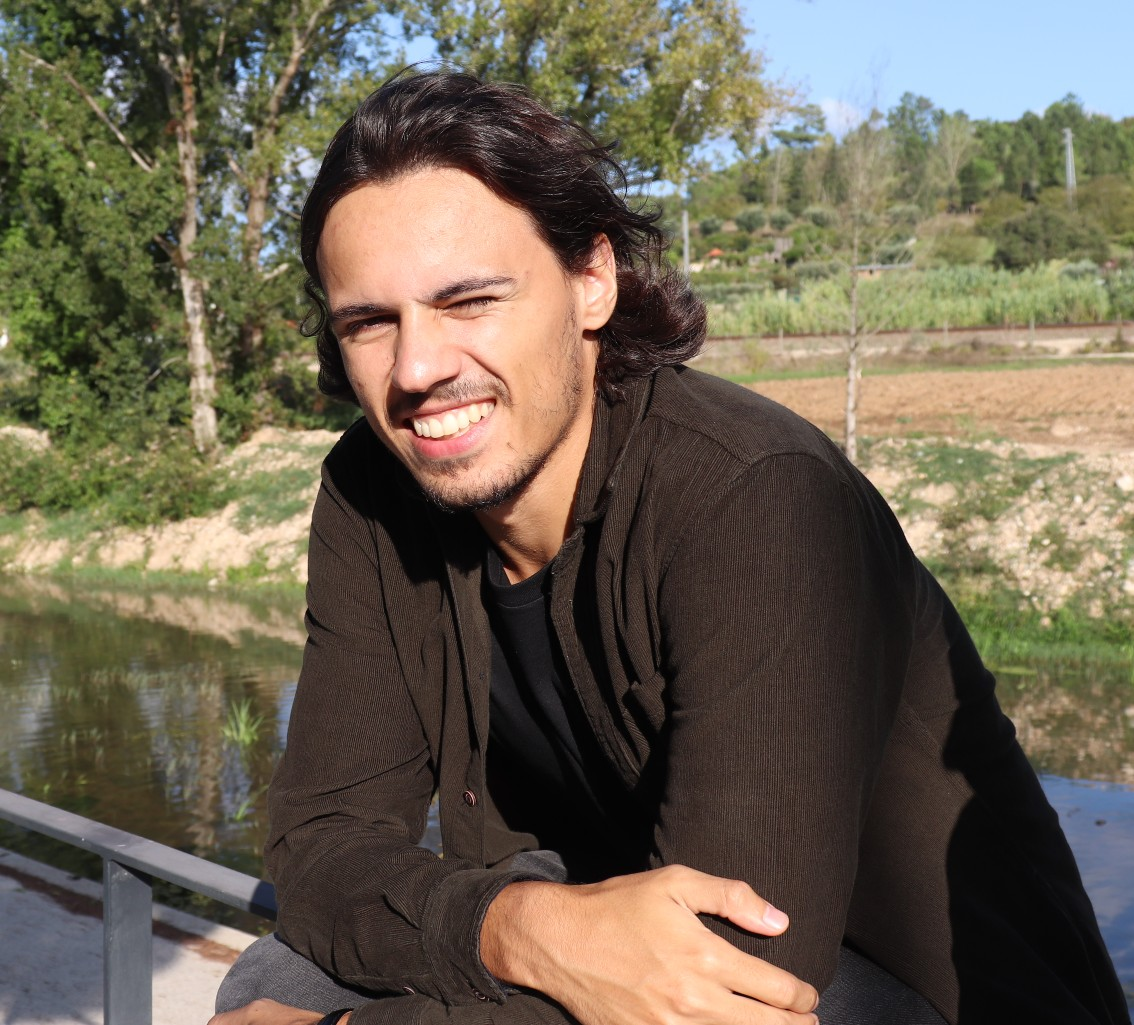
\includegraphics[width=0.6\columnwidth]{cv-photo.jpg}
	\vspace{-7cm}
\end{figure}

\begin{flushright}\small
	Diogo Fernandes \\
	\url{diogo.fernandes.12@hotmail.com}  \\
	\url{www.dimmaski.com} \\
\end{flushright}\normalsize
\framebreak


% Right frame
%%%%%%%%%%%%%%%%%%%%
\Huge\bfseries {\color{RoyalBlue} Diogo Fernandes} \\
\Large\bfseries  Software Engineer \\

\normalsize\normalfont

% About me
\begin{AboutMe}
Junior Software Engineer, that has been working as a Site Reliably Engineer for the past year. I'm interested in the CI/CD process, also a fan of immutable infrastructure and infrastructure as code. I'm looking for challenges that allow me to keep working on infrastructure but to write code at the same time.
\end{AboutMe}

% Experience
\CVSection{Experience}
\CVItem{Talkdesk Set. 2019 - present, Coimbra Portugal (Remote)}\\
Currently, I'm working in one of the R\&D clusters at TDX. Here, I'm learning about best practices with IAC, immutable infrastructure, and the CI/CD process. Working closely with the development teams, and also making sure that our infrastructure interfaces well with the rest of the company's.
\SmallSep

\CVItem{Ubiwhere Jul. 2019. - Set 2019, Coimbra Portugal}\\
Summer internship. Got to understand a bit more about ETL, python and docker. 
\SmallSep

\CVItem{Lifeguard Jun. 2016 - Set. 2019}\\
Worked in public pools and in a water park during my summer breaks throughout my bachelor's degree.
\SmallSep

\CVItem{Sonae Nov. 2015 - Apr. 2016, Pombal Portugal}\\
I worked as a baker after I quit my pilotage course in 2015. During this time I got more interested in Linux and the C programming language.
\SmallSep


\Sep

% Education
\CVSection{Education}
\CVItem{2016 - 2019, Universidade de Coimbra}\\
Bcs. Informatics Engineering 15/20
\SmallSep

\CVItem{2016 - 2016, Instituto Superior de Ciências da Informação e da Administração}\\
Lifeguard course.
\SmallSep

\CVItem{2015 - 2015, Escola Superior Náutica Infante D. Henrique
}\\
Bcs. Deck and Birdge Operations.
\SmallSep


% Skills
\CVSection{Tech Stack}

\CVItem{Daily use}
\begin{multicols}{3}
\begin{compactitem}[\color{RoyalBlue}$\circ$]
	\item Git
	\item Docker
	\item Ansible
	\item Terraform
	\item Python
	\item AWS
	\item Linux
\end{compactitem}
\end{multicols}
\Sep 

\CVItem{Other technologies}
\begin{multicols}{3}
\begin{compactitem}[\color{RoyalBlue}$\circ$]
	\item Drone CI
	\item Elasticsearch
	\item Jaeger tracing
	\item New Relic
	\item RabbitMQ
	\item Nomad
	\item Consul
\end{compactitem}
\end{multicols}
\Sep 

\end{document}

